In this section, the terminology and concepts utilized throughout the paper are defined. %The study is based on the Danish market for ancillary services, but the method presented here can be transferred to other markets.  

\subsection{Ancillary services provision from unconventional resources}\label{subsec:ASDER}
Ancillary services are utilized by transmission system operators (TSOs) to ensure a adequate and secure operation of the power system. 
%There is a variety of services targeting different aspects of the power system operation. 
%This work will focus solely on active power control, but the method presented here can be translated into other types of services, e.g. control of reactive power for voltage control. 
Currently, frequency containment reserve (primary reserve) and frequency restoration reserve (secondary reserves) \cite{entso1operational} are widely utilized by TSOs to ensure frequency stability. In the future, such services are expected to be delivered by aggregators \cite{pudjianto2007virtual,vrettos2015frequency}. Furthermore, with the introduction of aggregators, new possibilities arise for solving problems at distribution system level, e.g. congestion issues, leading to new flexibility services being defined for distribution system operators (DSOs), as presented in \cite{ding2013development}. %, which can also be delivered by aggregators. This work will present an examle of each type of service.  
%defines seven DSO-flexibility services, which can be traded through a flexibility clearing house (FLECH). Five of these concern active power regulations and two voltage management services. 

%\subsection{Flexible distributed energy resources} \label{sec:DERs}
%\kh{integrated this section with previous one}
With an increased electrification of the energy system due to the introduction of electric vehicles (EVs), heat pumps and local generation, DERs are expected to deliver an increasing amount of ancillary services in the future power grid. The DERs that can be utilized for ancillary services are those which can provide flexibility in consumption or generation without significantly impacting their primary energy service, e.g. battery state of charge and indoor temperature comfort \cite{costanzo2013coordination,halvgaard2012economic}.

%The incentive for a DER owner of contracting an aggregator to manage his flexibility will likely be economical by receiving a payment for his availability.
% However, the incentive could also be non-economical; for example, the aggregator could offer actual services to the DER owner, e.g. efficient operation of heat pumps by live monitoring of the coefficient of performance or provision of a web interface for indoor climate control, which allows the DER owner to control the indoor temperature in his home. % Another option could be that the aggregator controls a cluster of units owned by a single actor, e.g. the aggregator acts as a fleet operator for the optimal charging of a pool of EVs owned by single entity. 
%Similarly, it could also be in control of the heating of an office building, where the overall temperature of all offices should respect certain comfort bounds. In the following, such services will be referred to as asset management services (AMS). % \bondynote{Anders, you had a few ideas here didn't you?}

%Examples of relevant DERs are electrical vehicles, which can charge dynamically and achieve peak-shaving at the point of connection, while still respecting some overall performance requirements like a specific state of charge in the morning \cite{costanzo2013coordination}. An electrical heat pump for residential heating can in some situations during winter shift its consumption more than half a day to achieve an economic benefit for the owner as described in \cite{halvgaard2012economic}. Residential refrigerators can significantly reduce the frequency nadir by providing a fast reacting primary reserve, while secondary reserves can come from electric water heaters and heating, ventilation and air conditioning systems of commercial buildings as described in \cite{vrettos2015frequency}.
%\subsection{Congestion management and DSO services}
%It is anticipated that the DSOs will start to utilize flexibility in the future (ref).
%
%Different grid tariffs are alternatives to power system services (NEAS ref).

\subsection{Roles in the market for ancillary services}
%Denmark, 
Ancillary services are acquired in a single-buyer auction by a transmission system operator (TSO)\footnote{a European TSO corresponds largely to an ISO (independent system operator, with the limitation that a TSO does not  host the energy markets.} via an open market, where approved participants can bid their reserves.  Balance responsible parties (BRPs) are responsible for the balance of power production or consumption within their portfolio, with respect to the schedule of traded energy and the respective. The actors and their relationships can be seen in Fig.~\ref{fig:TSGmarket}.
Apart from the required approval, also a minimum bid size limits market entry, as most DERs have a smaller capacity \cite{koliou2014demand}. %\kh{that reference does not prove the point. need another one that compares bid size with entry level; like jason's http://drrc.lbl.gov/publications/demand-response-providing-ancillary  or this one (relevant earlier http://www.sciencedirect.com.globalproxy.cvt.dk/science/article/pii/S0360544209004034 ; or this one http://www.sciencedirect.com.globalproxy.cvt.dk/science/article/pii/S0360544214004800 .}. 

%Such market requirements further increases the need for 
Aggregators, who pool large numbers of DERs, can represent these as aggregate resource to a system operator. 
%Furthermore, most DER owners will likely not have the time, interest or knowledge to control their consumption 24 hours a day. 
%Because of this, a party called an Aggregator is needed, who pools a larger body of DER units and are responsible for the operation of these units. 
The aggregator can deliver TSO and DSO services as well as flexibility services for balance responsible parties (BRPs) e.g. \cite{tougaard2015flech,usef2015}.  
Finally, in order to avoid the aggregator creating imbalances for the Balance Responsible Consumer, all aggregator-service sales must occur through the Balance Responsible Consumer. 
\begin{figure}
  \centering
  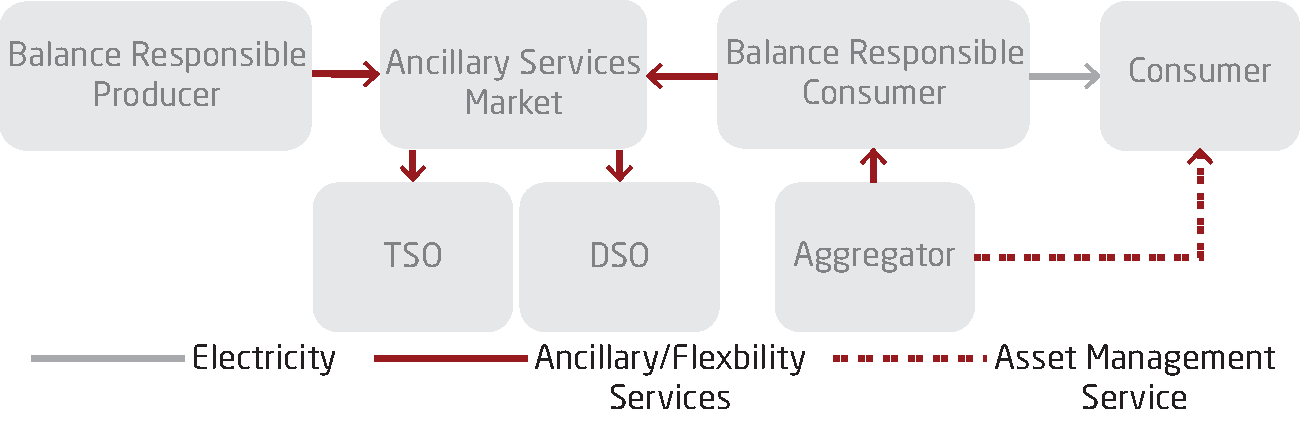
\includegraphics[width=\columnwidth]{graphics/tsg/market_future4}
  \caption{The new player in the market for ancillary services is the aggregator, which sells consumption flexibility on the ancillary service markets through the Balance Responsible Consumer. Some markets allow the aggregators to participate directly in the ancillary service markets with the condition that they coordinate with their Balance Responsible Consumer. It also provides flexibility services to BRPs and DSOs.}
  \label{fig:TSGmarket}
\end{figure}
%The aggregator will sign contracts with the DER owners and be the responsible party for delivery of service to the TSO, DSO or BRP. Further, the aggregator will have to ensure that certain performance parameters are respected towards the DER owner \cite{ding2013development}.
%Introduction of FLECH. \newline

\subsection{Service verification today}
When contracted for service, units are subject to a set of requirements. First, units must pass a prequalification test.% In PJM, when contracted for regulation, this consists of passing three consecutive tests.
Second, certified metering instrumentation must be installed on the unit, and telemetry equipment must be installed and connected to the system operator's Supervisory and Control Data Acquisition (SCADA) system.

For verifying reserve services, the system operator does random checks to see if the reserve is available at the unit \cite{EnerginetAncillary}. %\bondy{I'm not sure who to cite here... in ENDK AS document it is written that ENDK has the right to do random function checks, and that at any moment ENDK can ask for documentation of delivered service... but I've only had it from word of mouth that they actually sometimes do those random tests}\kh{but that's perfect - it's written that they can do it.}
With respect to regulation services, these are expected to be delivered within the required time requirements, and must be measured with acceptable accuracy. For example, for consumption units smaller than 1.5 MW acceptable accuracy is 2\% of the load \cite{Energinettek}.

%``service level agreements´´ etc.
%\kh{here should be a short outline of the actual service verification process; and how it's done today: pre-qualification, certified metering equipment on each generator , , then occasional (?) checks on the response; penalties for non-delivery, etc-}

\subsection{The need for service requirements modeling}\label{subsec:needforreq}
The concept of verification of ancillary services is moving towards a more flexible definition. Furthermore, new types of flexibility services are appearing, e.g. \cite{tougaard2015flech,heussen2013clearinghouse}. Part of the lessons learned from a demonstration of one of these new DSO services \cite{ipowerdemo,bondy2014powermax} is that the services, along with their requirements, need to be clearly defined if aggregators are to deliver them. The main problem being that the verification of services delivered by aggregators is complex.
%\hl{This is because it cannot be assumed that the services will be delivered by traditional (well understood) units, making verification more complex.} 
Also, research points at the need for change of the traditional service requirements if aggregators are to be enabled \cite{macdonald2012demand,koliou2014demand}. Thus, models that translate service contract requirements into benchmarks for performance assessment are needed.

From the market setup described in the previous section, parallels can be drawn to the concept of \emph{Service-Oriented Architectures} (SOAs) from the field of computer science. Under that paradigm, service is defined as: a logical representation of a repeatable business activity that has a specified outcome, is self-contained, may be composed of other services and is a \emph{black box} to consumers of the service \cite{opengroupsoa}. An element in SOAs are \emph{Standardized service contracts}, which contain service level agreements (SLAs). The SLAs can be interpreted as the requirements defined in an ancillary service contract. SLAs must define service performance metrics with corresponding service level objectives (SLOs), which are the agreed means for measuring performance.
%\kh{here motivate the need for formalized and generic requirements; good to use the iPower experience here as motivation}

PJM has established precedence in using performance metrics for verification of services. Their \emph{performance score} consists of a weighted average of three measures: delay, accuracy and precision. These measure the delay and correlation between the regulation signal and the reaction of the unit, and the difference in energy requested vs. energy supplied \cite{pjmperf}. These measures are tailored to the way frequency regulation is done at PJM (tracking of the regulation signal). Therefore, more general (and simple) models and performance metrics are needed to cover other frequency regulation services and the new flexibility services.
